\documentclass[11pt]{article}
\usepackage[review]{acl}
\usepackage{times}
\usepackage{latexsym}
\usepackage{booktabs}
\usepackage{amsmath}
\usepackage{amssymb}
\usepackage[T1]{fontenc}
\usepackage[utf8]{inputenc}
\usepackage{microtype}
\usepackage{graphicx}
\usepackage{enumitem}

\title{Whether a Relation Extractor Learns Argument Order\\
Depends on a Corpus Property Nobody Reports}

\author{Anonymous ACL submission}

\begin{document}
\maketitle

\begin{abstract}
A directional relation extractor should identify the same entity as subject whichever order the
pair is presented in. Nothing in standard practice enforces this, and we show that whether it
holds depends on a property of the training corpus that is never reported: the marginal
probability that the first-listed argument is the subject. Across three corpora we find that
when this prior is skewed ($0.708$) an unconstrained model takes the positional shortcut and
its swap consistency falls to $0.473$---below chance; when the prior is near balanced ($0.486$,
$0.544$) the model is forced to read content and reaches $0.94$--$0.97$, but never exactness.
Holding a corpus fixed and moving only this prior---reordering argument presentation and
nothing else---reproduces the effect on two benchmarks, and at a prior of $1.0$ swap
consistency is exactly $0$ while accuracy falls to precisely the test set's own positional
prior. The released state-of-the-art BioREDirect model sits at $0.700$ on its own benchmark,
where
$17.9\%$ of its directed predictions are returned unchanged under exchange---a
self-contradiction---and $16.7\%$ are abandoned to the undirected class.
We give two mechanisms that make the property exact rather than contingent. Canonicalising
argument order before encoding makes the two presentations byte-identical; an antisymmetric
readout $s(h_A,h_B) = g(h_A,h_B) - g(h_B,h_A)$, paired with a \emph{symmetric} directedness
score, makes it hold at every parameter setting given order-invariant encodings. The first is
what makes the property exact---to floating-point precision, whatever the head; the second
recovers most of it ($0.987$) when the encoder stays order-sensitive. Together they cost
$0.54\%$ of parameters and $2\%$ of throughput.
The guarantee is free rather than beneficial: direction accuracy is statistically
indistinguishable from the unconstrained arm on both public benchmarks
($0.911$ vs $0.912$ on BioRED, $p=0.79$; $0.963$ vs $0.966$ on
SemEval-2010 Task~8, $p=0.13$). We argue the right
way to obtain a property the evaluation convention already assumes is to construct it, not to
hope the corpus happens to supply it, and we release a swap-consistency protocol that needs no
new annotation and runs on any existing extractor.
\end{abstract}

\section{Introduction}
\label{sec:intro}

For directional relations, the label encodes an ordering: \emph{Cause-Effect(e1,e2)} and
\emph{Cause-Effect(e2,e1)} are distinct classes, and confusing them produces a knowledge-base
edge pointing the wrong way. The convention is near-universal, from SemEval-2010 Task~8
\citep{hendrickx2010semeval} through TACRED \citep{zhang2017position} and DocRED
\citep{yao2019docred} to recent biomedical work \citep{lai2025directionality}.

The convention carries an unstated assumption. The same pair can be presented in either order,
and the two presentations are semantically identical: if $A$ causes $B$ then presenting
$(B, A)$ must yield the mirrored label, so that the entity identified as subject does not
change. Nothing in the standard training objective enforces this. Each pair is seen in one
order during training and the model is never asked what it would say about the reverse.

We find that the property is therefore not reliably learned---and, more interestingly, that
whether it is learned at all depends on a property of the corpus that is never reported.
Write $\pi$ for the marginal probability that the first-listed argument is the subject. Across
three corpora with $\pi = 0.708$, $0.544$ and $0.486$, an unconstrained model trained on
order-sensitive input reaches swap consistency $0.473$, $0.938$ and $0.969$ respectively
(Figure~\ref{fig:pi}). When
$\pi$ is skewed the model takes the positional shortcut and performs \emph{below chance} on
consistency; when $\pi$ is balanced it is forced to read content and approximates the property
without ever attaining it. The released BioREDirect model \citep{lai2025directionality} sits at
$0.700$ on its own benchmark.

\begin{figure}[t]
\centering
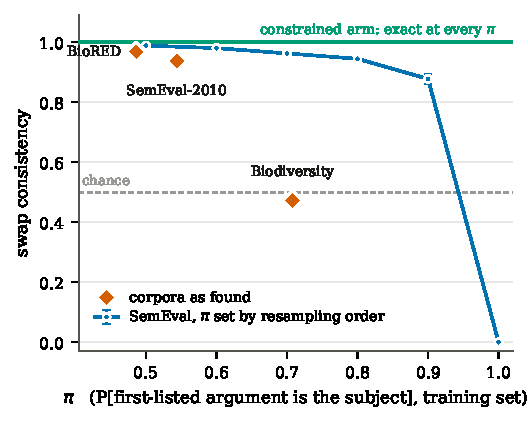
\includegraphics[width=\columnwidth]{fig/fig1_pi_consistency.pdf}
\caption{Swap consistency of an unconstrained model on order-sensitive input, against the
training corpus's positional prior $\pi$. The property is acquired only when the corpus
withholds the positional shortcut; at $\pi = 0.708$ it falls below chance. Bars span three
seeds (biodiversity is a single run). Our canonical arm is at $1.000$ for every $\pi$, by
construction rather than by training.}
\label{fig:pi}
\end{figure}

This reframes what the architecture is for. The property is not merely unenforced; it is
contingent on a corpus statistic that practitioners neither measure nor control. Constructing
it removes the contingency. We give two mechanisms that act at different points. The first
removes argument order from the encoder: sorting the two entities canonically before marking
them makes the two presentations byte-identical, so consistency holds exactly, for any readout.
The second constrains the readout: an antisymmetric head returns $s(h_A,h_B) = -s(h_B,h_A)$ at
every parameter setting, which delivers the property whenever the encodings it is given are
themselves order-invariant, and recovers most of it ($0.987$) when they are not. We pair the latter with a \emph{symmetric} directedness score, because whether a
relation is directed at all must \emph{not} change under exchange---a distinction a single
softmax over $\{$rightward, leftward, undirected$\}$ cannot express.

Our claims, each supported on more than one corpus:

\begin{enumerate}[noitemsep,topsep=2pt,leftmargin=*]
\item \textbf{Argument-order equivariance is contingent, not guaranteed}, and the contingency
      is predictable from a measurable corpus statistic
      (\S\ref{sec:res-contingency}) that \emph{causes} it: holding a corpus fixed and moving
      only the statistic reproduces the effect on two benchmarks
      (\S\ref{sec:res-intervention}).
\item \textbf{Exactness is cheap.} $0.54\%$ additional parameters, $2\%$ of throughput, holding
      to floating-point precision rather than approximately (\S\ref{sec:res-guarantee}).
\item \textbf{It is free.} Direction accuracy is statistically indistinguishable from the
      unconstrained arm on both public benchmarks (\S\ref{sec:res-accuracy}). We claim no
      accuracy benefit.
\end{enumerate}

We are explicit about what is not new. Separating relation identity from relation direction
dates to \citet{rink2010utd}. Antisymmetry by construction is standard in preference learning
\citep{burges2005ranknet,rigutini2011sortnet} and motivates several knowledge-graph embedding
models \citep{trouillon2016complex,sun2019rotate}. Placing a direction head on a shared encoder
is \citet{lai2025directionality}. What we have not found is an argument-order-invariant
\emph{input} for relation extraction: the field puts order into the label space, into role
markers \citep{zhou2021improved,soares2019matching}, or into a constrained permutation set
\citep{woo2022login}, rather than removing it from the encoder and recovering it at an
equivariant readout.

\section{Literature review}
\label{sec:related}

\paragraph{Direction in relation extraction.}
The dominant treatment folds direction into the label set. SemEval-2010 Task~8
\citep{hendrickx2010semeval} defines nine relation types in two argument orders plus
\emph{Other}; TACRED \citep{zhang2017position} and DocRED \citep{yao2019docred} order the
arguments in the instance instead. The winning SemEval system \citep{rink2010utd} already
factored the problem, using one classifier for relation type and a second, per type, for
direction, so the factorisation itself is not novel. What it lacks, and what we add, is any
invariance property: both stages see the arguments in text order and are free to exploit it.

\paragraph{Entity markers.}
Marking the arguments in the passage is standard and the punctuation we use is borrowed.
\citet{zhou2021improved} establish the typed entity marker in which the subject is enclosed in
\texttt{@} and the object in \texttt{\#}; \citet{soares2019matching} popularised the idea. We
invert the semantics: our markers denote \emph{positions in a canonical ordering}, not roles.
A reader familiar with the convention will otherwise assume the standard reading, under which
the invariance argument does not hold, so we flag the inversion explicitly.

\paragraph{Symmetry as an architectural constraint.}
Enforcing $f(a,b) = -f(b,a)$ by construction is old. RankNet \citep{burges2005ranknet} gives
$P(a \succ b) = 1 - P(b \succ a)$ identically; SortNet \citep{rigutini2011sortnet} enforces the
antisymmetry exactly by dual-neuron weight sharing and proves the constrained network remains a
universal approximator---a stronger result than the difference form we use. In knowledge-graph
embedding, the inability of symmetric scoring functions to represent antisymmetric relations
motivates ComplEx \citep{trouillon2016complex} and RotatE \citep{sun2019rotate}. Our
contribution is not the construction but its application: to a text encoder that must read
direction from a passage, paired with a symmetric score for undirectedness, and measured.

\paragraph{Invariance and equivariance.}
\citet{woo2022login}, in scene-graph generation, state the goal in the same vocabulary---%
equivariant under subject--object ordering while invariant to the permutation---and resolve it
in the opposite direction, by constraining the permutation set so the subject always precedes
the object. Frame averaging \citep{puny2022frame} is the general umbrella: our canonical sort
is a canonicalisation frame giving exact invariance, and our antisymmetric readout is group
averaging in the sign representation of $S_2$.

\paragraph{Shortcut learning and dataset artefacts.}
That models exploit superficial statistics rather than the intended signal is well documented
\citep{gururangan2018annotation,mccoy2019right,geirhos2020shortcut}. Our $\pi$ statistic is an
instance: a positional regularity that is invisible in standard reporting and that determines
whether an intended invariance is acquired. Partial-input baselines \citep{poliak2018hypothesis}
are the established diagnostic for the analogous problem in inference; our masked-passage
control (\S\ref{sec:res-accuracy}) plays that role here.

\paragraph{Consistency probes.}
Perturbing an input in a way that should have a predictable effect is established methodology
\citep{ribeiro2020checklist,elazar2021measuring}. \citet{yuan2025symmetry} show pretrained
encoders are at chance on a symmetry probe built by swapping subject and object in Wikidata
triples, and address it with symmetry-aware training objectives; we address it architecturally,
so no training signal is required. \citet{woo2022login} introduce a bidirectional diagnostic in
vision. Swap consistency (\S\ref{sec:method-metric}) is the analogue for directional relation
extraction and needs no new annotation.

\paragraph{Biomedical directional extraction.}
\citet{lai2025directionality} is our principal baseline. It adds $10{,}864$ manual
directionality annotations to BioRED \citep{luo2022biored} and predicts relation type, novelty
and direction from three heads on a shared encoder, with soft prompts and context chunking. Its
direction head is a four-way linear classifier over $\{$\emph{None}, \emph{Left\_to\_Right},
\emph{Right\_to\_Left}, \emph{No\_Direct}$\}$---confirmed here from the released weights---and
carries no symmetry constraint.

\section{Method}
\label{sec:method}

\subsection{Task and the property at issue}
\label{sec:method-task}
Given a passage $p$, an ordered pair of marked mentions $(x, y)$ and a relation type $t$,
predict whether the relation is directed and, if so, which of $x, y$ is its subject. Write
$\sigma(p, x, y, t) \in \{x, y, \varnothing\}$. The property is
\begin{equation}
\sigma(p, x, y, t) = \sigma(p, y, x, t),
\label{eq:consistency}
\end{equation}
a statement about the identity of the predicted subject, not about the label: the label must
mirror precisely so that the identified entity does not change.

\subsection{The corpus statistic $\pi$}
\label{sec:method-pi}
Let $\pi$ be the fraction of directed training instances whose \emph{first-listed} argument is
the subject. A model given order-sensitive input can always achieve accuracy
$\max(\pi, 1-\pi)$ by ignoring the passage. Where $\pi$ departs from $0.5$ this shortcut is
rewarded, and the intended content-based solution is correspondingly less necessary. $\pi$ is
trivially computable and, to our knowledge, never reported.

\subsection{Swap consistency}
\label{sec:method-metric}
We measure Eq.~\ref{eq:consistency} directly: construct the exchanged presentation of each test
pair, run the model on both, and record whether the same entity is named subject. The
construction is mechanical but must exchange \emph{every} slot in which the input encodes
order---role markers and any template stating the pair order.

It is easy to get wrong. Our first attempt on BioREDirect exchanged only the source and target
markers, leaving the question order intact, and reported $0.175$. That is an artefact: the
model reads the textual order of the entities rather than the marker labels, so the
manipulation changed the gold answer without changing the argument order of the input. The
corrected protocol exchanges both and gives $0.700$. We report the error because it is the
first thing a careful reader will probe.

\subsection{Two routes to exactness}
\label{sec:method-arch}
Let $h_A, h_B$ be the contextual representations of the marked spans and $c$ the sentence
representation.

\paragraph{Canonical input (invariance).}
Sort the two entity strings by a fixed total order---case-folded lexicographic---and mark the
first \texttt{@\,$\cdot$\,@} and the second \texttt{\#\,$\cdot$\,\#} in place. The token
sequence is then a function of the \emph{unordered} pair: the two presentations are
byte-identical and Eq.~\ref{eq:consistency} holds for any readout. Decoding to a label happens
outside the model, by comparing the \texttt{@}-marked entity to the first argument as given.
Canonicalisation also disarms $\pi$. Exactness does not depend on the canonical prior being
balanced---the two presentations are the same bytes whatever it is---but the shortcut also
stops paying, because which entity occupies the first slot is now decided by the alphabet
rather than by the corpus. Measured, the prior moves to $0.484$ on SemEval (from $0.544$) and
$0.502$ on BioRED (from $0.486$): alphabetical order carries essentially no information about
which argument is the subject, which is what makes it a usable canonical form.

\paragraph{Antisymmetric readout (equivariance).}
Independently of the input,
\begin{align}
s_{\mathrm{dir}} &= g([h_A; h_B; c; e_t]) - g([h_B; h_A; c; e_t]), \label{eq:antisym}\\
s_{\mathrm{und}} &= h([h_A; h_B; c; e_t]) + h([h_B; h_A; c; e_t]), \label{eq:sym}
\end{align}
with $e_t$ a small embedding of the relation type and $g, h$ two-layer networks.
Eq.~\ref{eq:antisym} is exactly antisymmetric and Eq.~\ref{eq:sym} exactly symmetric, at every
parameter setting, before and during training.

The pairing carries the argument. \emph{Which} entity is the subject must invert under
exchange; \emph{whether the relation is directed at all} must not. A single softmax over
$\{$rightward, leftward, undirected$\}$ expresses neither constraint: exchanging the arguments
can move mass between rightward and leftward \emph{and} into or out of undirected, so the model
may hold two incompatible beliefs about one pair. We verify both properties numerically before
training; residuals are $0$ to machine precision.

\paragraph{Keeping the relation out of the encoder.}
The relation type enters only at the head, through $e_t$; the encoder never sees the relation
string. This makes the invariance argument airtight---direction cannot re-enter through the
relation surface form---and lets one small head serve every relation in the schema.

\subsection{Model, cost and protocol}
\label{sec:method-cost}
The encoder is BiomedBERT-base \citep{gu2021domain} in all arms. The direction head is
$594{,}465$ parameters, $0.54\%$ of the encoder, costing $2\%$ of CPU throughput ($33.0$
against $33.8$ pairs/s on eight threads). Arms within a comparison share encoder, optimiser,
schedule, epochs and data, differing only on the axis under test. We report means over three
seeds.

\subsection{Corpora}
\label{sec:method-data}
\textbf{BioRED} \citep{luo2022biored} with the directionality annotations of
\citet{lai2025directionality}: $1{,}163$ test pairs carrying a relation, $1{,}045$ directed
($527$/$518$) and $118$ undirected; $\pi = 0.486$. Clean mentions and passages are recovered
from the PubTator source, using the smallest sentence window containing both entities as the
baseline's own chunking does.

\textbf{SemEval-2010 Task~8} \citep{hendrickx2010semeval}: $7{,}991$ training and $2{,}713$
test instances after removing pairs with identical mention strings; $2{,}260$ directed test
instances and $453$ \emph{Other}, treated as undirected. General domain. $\pi = 0.544$.

\textbf{Biodiversity verification set}: $437$ expert-graded candidate triples from a deployed
literature-mining pipeline, plus $84$ human-annotated direction items over $79$ relation
surface forms. $\pi = 0.708$---the skewed case. Small, and treated accordingly.

\section{Results}
\label{sec:results}

\subsection{Equivariance is contingent on $\pi$}
\label{sec:res-contingency}
Table~\ref{tab:contingency} and Figure~\ref{fig:pi} are the central result. An unconstrained model on order-sensitive
input---standard practice---acquires the equivariance only when the corpus forces it to. At
$\pi = 0.708$ the positional shortcut is available and consistency falls to $0.473$, below
chance. At $\pi \approx 0.5$ the shortcut is worthless and consistency reaches $0.94$--$0.97$,
but never $1$.

We derived this relationship from the biodiversity and BioRED corpora and used it to predict
SemEval before running it: at $\pi = 0.544$, mildly skewed, consistency should fall between and
nearer the balanced end. It does.

\begin{table}[t]
\centering\small
\begin{tabular}{lccc}
\toprule
Corpus & $\pi$ & Uncon.\ swap & Ours \\
\midrule
Biodiversity & 0.708 & 0.473 & 1.000 \\
SemEval-2010 & 0.544 & 0.938 & 1.000 \\
BioRED       & 0.486 & 0.969 & 1.000 \\
\midrule
\multicolumn{2}{l}{BioREDirect (released)} & 0.700 & --- \\
\bottomrule
\end{tabular}
\caption{Swap consistency of the order-sensitive unconstrained arm against the training-corpus
prior $\pi$, with our canonical arm for reference.}
\label{tab:contingency}
\end{table}

\subsection{$\pi$ causes it: a controlled intervention}
\label{sec:res-intervention}
Three corpora with a mechanism attached is still an observation. To make the claim causal we
hold the corpus fixed and move $\pi$ directly. For a target $\pi$ we rewrite the SemEval
training set by changing \emph{only the order in which the two arguments are presented},
flipping a chosen subset of pairs. The passages, the pairs, the relation types, the gold
subjects and the test set are all untouched---the generator asserts that the pair multiset, the
passages and the directedness flags are unchanged before it writes---so $\pi$ is the single
manipulated variable. Two seeds per point.

Table~\ref{tab:sweep} and Figure~\ref{fig:sweep} give the result. Swap consistency falls
monotonically with $\pi$, from $0.989$ at $0.50$ to $0.878$ at $0.90$, while direction accuracy
barely moves. That gap is the practical warning in one line: between $\pi = 0.5$ and
$\pi = 0.9$ a model loses eleven points of consistency for three points of accuracy, so a
leaderboard reporting accuracy would show almost nothing wrong.

\begin{table}[t]
\centering\small
\begin{tabular}{lccc}
\toprule
$\pi$ & Dir.\ acc. & Swap & BioRED swap \\
\midrule
0.50 & 0.9608 & 0.9889 & 0.9842 \\
0.60 & 0.9604 & 0.9805 & --- \\
0.70 & 0.9582 & 0.9628 & 0.9732 \\
0.80 & 0.9502 & 0.9449 & --- \\
0.90 & 0.9272 & 0.8779 & 0.8789 \\
1.00 & \textbf{0.5845} & $\mathbf{0.0000}$ & --- \\
\midrule
\multicolumn{4}{l}{\emph{canonical $+$ symmetric, same training sets}} \\
0.50 & 0.9646 & $\mathbf{1.0000}$ & --- \\
1.00 & 0.9650 & $\mathbf{1.0000}$ & --- \\
\bottomrule
\end{tabular}
\caption{$\pi$ imposed on the training set by reordering argument presentation and nothing
else. Two seeds per point; standard deviations are at most $0.017$, and both seeds of every
point are in Appendix~\ref{app:sweep}.}
\label{tab:sweep}
\end{table}

\begin{figure}[t]
\centering
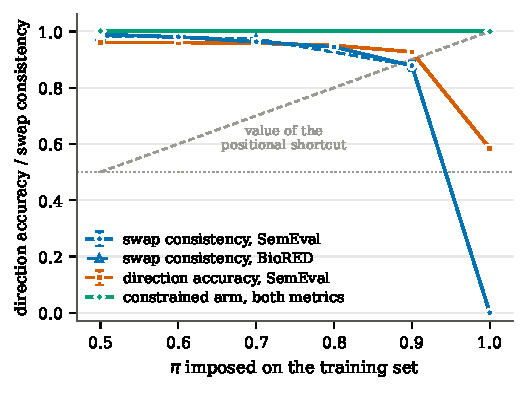
\includegraphics[width=\columnwidth]{fig/fig2_pi_sweep.pdf}
\caption{The same corpus at six priors. Consistency degrades while accuracy holds, until the
shortcut becomes worth more than reading the passage. The constrained arm, trained on the same
data, is flat at $1.000$ at both extremes.}
\label{fig:sweep}
\end{figure}

The endpoint is unambiguous. At $\pi = 1.00$, where every training pair is presented
subject-first, swap consistency is exactly $0.0000$: the model names the first-listed entity
every time, so exchanging the arguments always changes its answer. Its accuracy is $0.5845$,
which is exactly the test set's own positional prior to four decimal places---the signature of
a model that has learned the shortcut and nothing else. Trained on the identical data, the
canonical arm is untouched: $0.9650$ accuracy and $1.000$ consistency at $\pi = 1.00$ against
$0.9646$ and $1.000$ at $\pi = 0.50$. Immunity to the corpus's positional prior is what the
construction buys.

Repeating the manipulation on BioRED reproduces the curve ($0.984 \rightarrow 0.973 \rightarrow
0.879$ at $\pi = 0.50, 0.70, 0.90$), so the effect is not a property of one dataset.

\paragraph{$\pi$ sets the price, not the outcome.} One comparison refines the account. SemEval
forced to $\pi = 0.70$ keeps consistency at $0.963$, whereas the biodiversity corpus at its
natural $\pi = 0.708$ collapses to $0.473$. $\pi$ therefore fixes what the shortcut is
\emph{worth}---$\max(\pi, 1-\pi)$ on the training distribution---but whether the model takes it
depends on what reading the passage is worth instead. In SemEval a content solution is worth
$0.966$ against a $0.70$ shortcut and wins easily. In the biodiversity data the best content
solution we obtain is $0.869$, and the relation surface form adds almost nothing on top of
position: a lookup table from the relation form predicts the subject at $0.7152$ against
$0.7075$ for answering ``first-listed'' unconditionally. The shortcut is nearly competitive
with everything else available, and it wins. The sweep shows the same crossover within a single
corpus: SemEval degrades gently while the shortcut is worth less than $0.966$, and collapses
once it is worth more.

\subsection{What the failure looks like}
\label{sec:res-inconsistency}
On the released BioREDirect model, of the $854$ BioRED test pairs for which it predicts a
direction, $65.3\%$ are correctly mirrored under exchange, $17.9\%$ are returned
unchanged---naming a different entity as subject depending on presentation order---and $16.7\%$
are abandoned to the undirected class.

The failure is specific. Relation detection barely moves under exchange
($\mathrm{F}_1\ 0.7926 \rightarrow 0.7861$) while relation-plus-direction falls
$0.5550 \rightarrow 0.4013$. What the model knows about \emph{whether} two entities are related
survives; what it knows about \emph{which way} does not.

\subsection{The guarantee holds exactly}
\label{sec:res-guarantee}
Across every arm using canonical input, swap consistency is $1.000$ and the maximum deviation
between a prediction and its mirror is $2.98\times10^{-8}$---floating-point precision, not
approximation. This holds whichever head sits on top, because the encoder receives identical
bytes in both presentations.

The antisymmetric readout does not by itself deliver the same thing, and it is worth being
exact about why. Eq.~\ref{eq:antisym} is antisymmetric in its two arguments at every parameter
setting, so it guarantees the property \emph{conditional on} $h_A$ and $h_B$ being unchanged by
the exchange. An order-sensitive encoder breaks that condition: it genuinely sees different
tokens when the markers move, so $h_A$ and $h_B$ are not the same vectors. Empirically the head
recovers most of the gap but never closes it---$0.987 \pm 0.002$ on SemEval against $0.938 \pm
0.028$ for the unconstrained head, and $0.969$ on the biodiversity set against $0.473$. The two
mechanisms are therefore not interchangeable: canonicalisation is what makes the property
exact, and the antisymmetric head is what makes it nearly free to approximate when
canonicalisation is unavailable---for instance where argument order carries information the
task needs.

\subsection{Accuracy: the guarantee is free}
\label{sec:res-accuracy}
Table~\ref{tab:main} gives the head-to-head. On both public benchmarks the canonical-symmetric
arm and the order-sensitive unconstrained arm are indistinguishable. Summarising each arm by the
majority vote of its three seeds and comparing per item, the unconstrained arm is nominally
ahead on both---by $0.002$ on BioRED ($6$ vs $8$ discordant items, McNemar with continuity
correction $p=0.79$) and by $0.004$ on SemEval ($13$ vs $23$ discordant, $p=0.13$)---and neither
gap approaches significance. \textbf{We claim no accuracy benefit from the construction}; we
claim it costs nothing.

The $0.766$ of the released BioREDirect model is not directly comparable to either arm: it
performs a joint task (relation, novelty, direction) with soft prompts and multi-chunk pooling,
so the gap reflects system configuration rather than the design axis under test. We report it
for context, not as evidence for our design.

\begin{table}[t]
\centering\small
\begin{tabular}{llcc}
\toprule
Corpus & Arm & Dir.\ acc. & Swap \\
\midrule
BioRED & BioREDirect (released) & 0.766 & 0.700 \\
       & text $+$ unconstrained & 0.912 & 0.969 \\
       & \textbf{canonical $+$ sym.} & 0.911 & $\mathbf{1.000}$ \\
\midrule
SemEval & text $+$ unconstrained & 0.966 & 0.938 \\
        & \textbf{canonical $+$ sym.} & 0.963 & $\mathbf{1.000}$ \\
\bottomrule
\end{tabular}
\caption{Direction accuracy on gold-directed pairs and swap consistency. All BioRED and
SemEval figures are means over three seeds; per-seed values are in
Appendices~\ref{app:seeds} and~\ref{app:sweep}.}
\label{tab:main}
\end{table}

Two controls support that the models read the passage rather than exploiting surface
regularities. Withholding the relation type entirely changes BioRED accuracy from $0.909$ to
$0.910$, so the head does not lean on that feature. Masking the passage and presenting only the
two entity names drops the biodiversity direction model to $0.464$---chance---so it is not
recalling which entities typically stand in which role.

\subsection{Decomposing the two mechanisms}
\label{sec:res-ablation}
Table~\ref{tab:ablation} isolates each design choice, on the skewed biodiversity set where the
distinction bites and on SemEval, where three seeds per cell and a 453-instance undirected
class make the comparison stable.

The design separates into two main effects with no interaction. \textbf{Consistency is decided
by the input format}: both canonical cells are exactly $1.000$, and neither text cell reaches
it whatever the head. \textbf{Undirectedness is decided by the head}: on SemEval the symmetric
branch gains $\approx 0.043$ AUC under both input formats. \textbf{Accuracy is decided by
neither}: the four SemEval cells span $0.0036$, within about two standard deviations of seed
noise, and on biodiversity no difference reaches significance at $n=84$ (canonical input
$p=0.239$; symmetric head $p=1.000$).

One result does not replicate. On the 84-item set the unconstrained head looks like the better
undirectedness detector ($0.811$ vs $0.748$); on SemEval that reverses cleanly and
consistently. The biodiversity set has too few undirected items to support the comparison, and
we report the disagreement rather than the convenient half of it.

\begin{table}[t]
\centering\small
\begin{tabular}{llccc}
\toprule
Input & Head & Acc. & Und.\ AUC & Swap \\
\midrule
\multicolumn{5}{l}{\emph{Biodiversity}, $n=84$, $\pi=0.708$, one run} \\
canon. & sym.   & \textbf{0.869} & 0.748 & \textbf{1.000} \\
canon. & uncon. & 0.857 & 0.787 & \textbf{1.000} \\
text   & sym.   & 0.810 & 0.718 & 0.969 \\
text   & uncon. & 0.786 & \textbf{0.811} & 0.473 \\
\midrule
\multicolumn{5}{l}{\emph{SemEval}, $n=2{,}260$, $\pi=0.544$, 3 seeds} \\
canon. & sym.   & 0.9625 & \textbf{0.947} & $\mathbf{1.0000}$ \\
canon. & uncon. & 0.9634 & 0.904 & $\mathbf{1.0000}$ \\
text   & sym.   & \textbf{0.9661} & 0.947 & 0.9869 \\
text   & uncon. & 0.9658 & 0.907 & 0.9383 \\
\bottomrule
\end{tabular}
\caption{Design ablation on both corpora. Canonical input fixes swap consistency at floating-point
exactness; the symmetric head fixes undirectedness detection; neither moves accuracy. SemEval
figures are means over three seeds; per-seed values are in Appendix~\ref{app:seeds}.}
\label{tab:ablation}
\end{table}

\subsection{The applied setting}
\label{sec:res-applied}
On the biodiversity verification set the same model raises $\mathrm{F}_1$ from $0.816$ to
$0.902$ against a deployed sentence-level filter's own recorded decisions (McNemar
$p = 2.3\times10^{-4}$, $437$ items) at unchanged inference cost. The honest characterisation
is robustness to prevalence shift rather than raw accuracy: across blocks spanning prevalence
$0.31$ to $0.85$, one fixed threshold gives an $\mathrm{F}_1$ spread of $0.070$ against the
filter's $0.169$.

\section{Discussion and conclusion}
\label{sec:discussion}

The measurement is the part we would most like reused. It costs nothing---no annotation, no
retraining, one extra forward pass over an existing test set---and on the evidence here it is
worth running on any released directional extractor.

The finding it produces is not that published systems are careless. It is that a property the
evaluation convention silently assumes is delivered only when the corpus happens to make the
alternative unprofitable. $\pi$ is trivial to compute, is not reported in any dataset paper we
examined, and predicts whether the intended invariance will be acquired. A corpus with a skewed
positional prior will produce models that look accurate and are incoherent under exchange; a
balanced one will not, and neither the model card nor the leaderboard will distinguish them.

The architectural response is modest in isolation and we have said so. The factorisation is
\citeauthor{rink2010utd}'s; the antisymmetric construction is \citeauthor{rigutini2011sortnet}'s;
the markers are \citeauthor{zhou2021improved}'s with the semantics inverted. What is new is the
combination, the measurement that motivates it, and the observation that the property is
otherwise left to chance.

Two findings cut against a clean story and belong in the record. The first is a disagreement
between our two ablations. On the $84$-item biodiversity set the unconstrained head detects
undirectedness \emph{better} than ours, which we first read as the symmetry constraint costing
flexibility in the undirected class; on SemEval, with $453$ undirected instances and three
seeds per cell, the effect reverses cleanly and the symmetric branch wins by $0.043$ AUC under
both input formats. We take the larger measurement to be the reliable one and report the
smaller because it is what a $n=84$ ablation can do to a conclusion. The second is that no
accuracy difference between design cells is significant on either corpus---only the
consistency differences are structural, and that is the whole claim.

\paragraph{Limitations.}
The human direction gold for the applied setting is $84$ items: enough to show the head reads
the passage, not enough to separate it from a good dependency-parse rule, which we estimate
would need on the order of $2{,}700$ annotations. BioREDirect performs a joint task while our
arms perform direction given the pair; we control for the most obvious confound
(\S\ref{sec:res-accuracy}) but not all, and we therefore do not treat that comparison as
evidence for the design. Our context window is the infix span where the baseline uses prefix,
suffix and infix with max-pooling. The $\pi$ relationship is established by controlled
manipulation on two corpora and observed on a third; what the intervention does not settle is
the functional form, since six points on one corpus and three on another constrain the shape
only loosely, nor how $\pi$ interacts with the many other ways a corpus can differ. Finally, the
curated relation vocabulary shows that many relation surface forms carry no direction at
all---$12$ of $79$ annotated forms were marked undirected by the curator---so direction is
defined only on a subset of extracted edges, and a system reporting it everywhere is
overclaiming.

\bibliography{references}
\bibliographystyle{acl_natbib}

\appendix

\section{Per-seed values}
\label{app:seeds}
Table~\ref{tab:seeds} gives every seed behind the SemEval means in
Table~\ref{tab:ablation}. Swap consistency for the two canonical cells is exactly $1.0000$ in
every run; the largest deviation between any prediction and its mirror is
$2.98\times10^{-8}$ across all six, which is the resolution of the float comparison rather
than a measured discrepancy. The undirectedness AUC carries the largest seed variance of any
quantity we report ($\sigma \approx 0.02$--$0.03$), which is why the head effect is stated as a
difference of means over three seeds rather than from a single run: on seed~1 alone it would
have read as $0.98$ against $0.93$, roughly twice its stable size.

\begin{table}[h]
\centering\small
\begin{tabular}{llllll}
\toprule
Input & Head & & s1 & s2 & s3 \\
\midrule
canon. & sym.   & acc  & 0.9650 & 0.9615 & 0.9611 \\
       &        & swap & 1.0000 & 1.0000 & 1.0000 \\
       &        & AUC  & 0.9823 & 0.9245 & 0.9354 \\
\midrule
canon. & uncon. & acc  & 0.9642 & 0.9624 & 0.9637 \\
       &        & swap & 1.0000 & 1.0000 & 1.0000 \\
       &        & AUC  & 0.9297 & 0.8865 & 0.8951 \\
\midrule
text   & sym.   & acc  & 0.9668 & 0.9681 & 0.9633 \\
       &        & swap & 0.9894 & 0.9863 & 0.9850 \\
       &        & AUC  & 0.9794 & 0.9238 & 0.9365 \\
\midrule
text   & uncon. & acc  & 0.9642 & 0.9673 & 0.9659 \\
       &        & swap & 0.9588 & 0.9066 & 0.9496 \\
       &        & AUC  & 0.9298 & 0.8952 & 0.8962 \\
\bottomrule
\end{tabular}
\caption{SemEval-2010 Task~8, all three seeds per cell.}
\label{tab:seeds}
\end{table}

\begin{table}[h]
\centering\small
\begin{tabular}{llccc}
\toprule
Arm & & s1 & s2 & s3 \\
\midrule
canon.\ $+$ sym. & acc  & 0.9091 & 0.9100 & 0.9129 \\
                 & swap & 1.0000 & 1.0000 & 1.0000 \\
\midrule
text $+$ uncon.  & acc  & 0.9120 & 0.9129 & 0.9100 \\
                 & swap & 0.9809 & 0.9694 & 0.9569 \\
\bottomrule
\end{tabular}
\caption{BioRED test, $1{,}045$ gold-directed pairs, all three seeds.}
\label{tab:seedsbiored}
\end{table}

\section{Per-seed values for the $\pi$ intervention}
\label{app:sweep}
Table~\ref{tab:seedssweep} gives both seeds of every point in Table~\ref{tab:sweep}. The
$\pi = 1.00$ row is worth noting: the two seeds agree to four decimals on both metrics, which
is what a degenerate solution looks like---there is only one way to answer ``first-listed''
every time, so independent initialisations land on identical behaviour rather than merely
similar behaviour.

\begin{table}[h]
\centering\small
\begin{tabular}{llcccc}
\toprule
 & & \multicolumn{2}{c}{accuracy} & \multicolumn{2}{c}{swap} \\
\cmidrule(lr){3-4}\cmidrule(lr){5-6}
Corpus & $\pi$ & s1 & s2 & s1 & s2 \\
\midrule
SemEval & 0.50 & 0.9611 & 0.9606 & 0.9925 & 0.9854 \\
        & 0.60 & 0.9593 & 0.9615 & 0.9832 & 0.9779 \\
        & 0.70 & 0.9580 & 0.9584 & 0.9597 & 0.9659 \\
        & 0.80 & 0.9478 & 0.9527 & 0.9420 & 0.9478 \\
        & 0.90 & 0.9226 & 0.9319 & 0.8659 & 0.8898 \\
        & 1.00 & 0.5845 & 0.5845 & 0.0000 & 0.0000 \\
\midrule
BioRED  & 0.50 & 0.9053 & 0.9062 & 0.9866 & 0.9818 \\
        & 0.70 & 0.9072 & 0.9072 & 0.9780 & 0.9684 \\
        & 0.90 & 0.8842 & 0.8813 & 0.8746 & 0.8833 \\
\bottomrule
\end{tabular}
\caption{The controlled $\pi$ sweep, both seeds.}
\label{tab:seedssweep}
\end{table}

\end{document}
